\documentclass[14pt]{extarticle}
\usepackage[utf8]{inputenc}
\usepackage[margin=0.5in]{geometry}
\usepackage{amssymb}
\usepackage{amsmath}
\usepackage{pgfplots}
\pgfplotsset{width=10cm,compat=1.9}
\usepackage{mathtools}
\usepackage{graphicx}


\DeclarePairedDelimiter\abs{\lvert}{\rvert}%
\DeclarePairedDelimiter\norm{\lVert}{\rVert}%
\newcommand{\taninv}{\tan^{-1}}


\title{Matemáticas para las Ciencias Aplicadas $||$ \\ Profesor: Hector (Awakatito) Díaz}
\author{Santiago Arroyo Lozano}
\date{Abril 3 2020}

\begin{document}

\maketitle

\section{En los siguientes ejercicios, exprese cada vector en términos de su magnitud y de su ángulo de dirección: \\ $\vec{a} = \norm{\vec{a}}(\cos{\theta},\sin{\theta})$}
    Propiedades a tomar en cuenta: \\
     $\vec{a} = (x,y)$ \\
     $\norm{\vec{a}} = \sqrt{x^2+y^2}$ \\
     $\theta = \taninv{\left(\frac{co}{ca}\right)}$ \\ \\
    Esto lo sabemos por que al formar el vector lo podemos ver también como: \\
    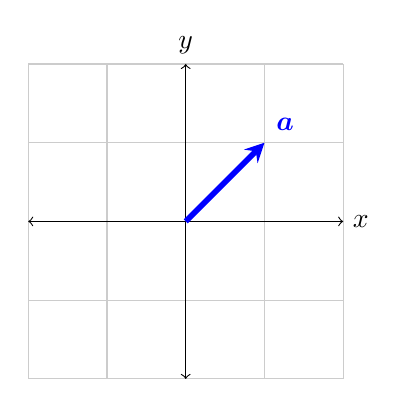
\begin{tikzpicture}
            \draw[thin,gray!40] (-2,-2) grid (2,2);
            \draw[<->] (-2,0)--(2,0) node[right]{$x$};
            \draw[<->] (0,-2)--(0,2) node[above]{$y$};
            \draw[line width=2pt,blue,-stealth](0,0)--(1,1) node[anchor=south west]{$\boldsymbol{a}$};
        \end{tikzpicture}
        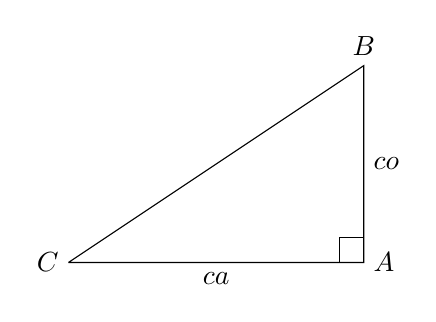
\begin{tikzpicture}[scale=1.25]%,cap=round,>=latex]
            \coordinate [label=left:$C$] (A) at (-1.5cm,-1.cm);
            \coordinate [label=right:$A$] (C) at (1.5cm,-1.0cm);
            \coordinate [label=above:$B$] (B) at (1.5cm,1.0cm);
            \draw (A) -- node[above] {} (B) -- node[right] {$co$} (C) -- node[below] {$ca$} (A);
            \draw (1.25cm,-1.0cm) rectangle (1.5cm,-0.75cm);
        \end{tikzpicture} \\
        Donde el Cateto Opuesto y el Cateto Adyacente pueden tomar los valores positivos de $x$ o $y$. Siendo la hipotenusa el vector $\vec{a}$. Que se muestra a la izquierda del triangulo ABC.
    \subsection{$(\sqrt{3},1)$}
        Como en este caso el Cateto Opuesto es el valor de la magnitud $x$, osease $1$, el Cateto Adyacente es $\sqrt{3}$
        \begin{align}
            \notag \theta &= \taninv{\left(\frac{1}{\sqrt{3}}\right)} = 30° \\ \notag \\
            \notag \norm{\vec{a}} &= \sqrt{\sqrt{3}^2+1^2} = \sqrt{3+1} \\
            \notag &= \sqrt{4} = 2
        \end{align}
        El vector se representa como
        \begin{align}
           \notag (\sqrt{3},1) = 2(\cos30,\sin30)
        \end{align}
    \subsection{($1$,$-2\sqrt{2}$)}
         Como en este caso el Cateto Opuesto es el valor de la magnitud $x$, osease $1$, el Cateto Adyacente es $2\sqrt{2}$, Cambiamos valores negativos en la tangente a positivos
        \begin{align}
            \tag{Como estamos en el tercer cuadrante se suman $270°$} \theta &= 270 + \taninv{\left(\frac{1}{2\sqrt{2}}\right)} \\
            \notag &= 270 + 19.47 = 289.47°
        \end{align}
        \begin{align}
            \notag \norm{\vec{a}} &= \sqrt{1^2+(-2\sqrt{2})^2} = \sqrt{1+8} \\
            \notag &= \sqrt{9} = 3
        \end{align}
        El vector se representa como
        \begin{align}
           \notag (1,-2\sqrt{2}) = 3(\cos289.47,\sin289.47)
        \end{align}
    \subsection{($3$, $-5$)}
        Como en este caso el Cateto Opuesto es el valor de la magnitud $x$, osease $3$, el Cateto Adyacente es $5$
        \begin{align}
            \tag{Como estamos en el tercer cuadrante se suman $270°$} \theta &= 270 + \taninv{\left(\frac{3}{5}\right)} \\
            \notag &= 270 + 30.96 = 300.96°
            \end{align}
        \begin{align}
            \notag \norm{\vec{a}} &= \sqrt{3^2+(-5)^2} = \sqrt{9+25} \\
            \notag &= \sqrt{34}
        \end{align}
        El vector se representa como
        \begin{align}
           \notag (3,-5) = \sqrt{34}(\cos300.96,\sin300.96)
        \end{align}
    \subsection{$\sqrt{7}$,$3$}
    Como en este caso el Cateto Opuesto es el valor de la magnitud $y$, osease $3$, el Cateto Adyacente es $\sqrt{7}$
        \begin{align}
            \notag \theta &= \taninv{\left(\frac{3}{\sqrt{7}}\right)} = 48.59°
        \end{align}
        \begin{align}
            \notag \norm{\vec{a}} &= \sqrt{9\sqrt{7})^2+3^2} = \sqrt{7+9} \\
            \notag &= \sqrt{16} = 4
        \end{align}
        El vector se representa como
        \begin{align}
           \notag (\sqrt{7},3) = 4(\cos48.59,\sin48.59)
        \end{align}
\section{En los siguientes ejercicios, encuentre un vector unitario perpendicular al vector dado (Le llamaremos $\vec{a}$ a cada vector dado}
Propiedades a tomar en cuenta: \\
Un vector $\vec{v}$ es perprendicular a $\vec{a}$ si $\vec{a}\cdot\vec{v} = 0$  \\
Sabemos que si tenemos el vector $(x,y)$ basta con intercambiar los valores y vambiar el signo de uno de ellos para encontrar un vector perpendicular. Ejemplos: $(-y,x),(y,-x)$ \\  \\
$\frac{\vec{v}}{\norm{\vec{v}}}$ siempre es un vector unitario \\ \\
Como podemos ver en la siguiente imagen, como B es un vector perpendiular a A, entonces el vector unitario Au es un vector unitario de A perpendicular a B. Entonces basta con encontrar un vector perpendicular y hacerlo un vector unitario \\
\includegraphics{vector.png}
    \subsection{($2$,$-2\sqrt{3}$)}
        Un vector perpendicular a $\vec{a}$ es $\vec{v} = (2\sqrt{3},2)$
        \begin{align}
            \notag \norm{\vec{v}} &= \sqrt{(2\sqrt{3})^2+2^2} = \sqrt{4\cdot 3 + 4} \\
           \notag &= \sqrt{16} = 4
         \end{align}
        $\therefore \left(\frac{2\sqrt{3}}{4}, \frac{2}{4}\right)$ es un vector unitario perpendicular a $\vec{a}$
    \subsection{($0$,$-4$)}
        Un vector perpendicular a $\vec{a}$ es $\vec{v} = (4,0)$
        \begin{align}
            \notag \norm{\vec{v}} = \sqrt{4^2+0^2} = \sqrt{16} = 4
        \end{align}
         $\therefore \left(\frac{4}{4}, \frac{0}{4}\right)$ es un vector unitario perpendicular a $\vec{a}$
    \subsection{($a$,$b$)}
        Un vector perpendicular a $\vec{a}$ es $\vec{v} = (-b,a)$
        \begin{align}
            \notag \norm{\vec{v}} &= \sqrt{(-b)^2+a^2} = \sqrt{b^2+a^2}
         \end{align}
        $\therefore \left(\frac{-b}{\sqrt{b^2+a^2}}, \frac{a}{\sqrt{b^2+a^2}}\right)$ es un vector unitario perpendicular a $\vec{a}$
    \subsection{($a$,$2a$)}
         Un vector perpendicular a $\vec{a}$ es $\vec{v} = (2a,-a)$
        \begin{align}
            \notag \norm{\vec{v}} &= \sqrt{(2a)^2+(-a)^2} = \sqrt{4a^2+a^2} \\
            \notag &= \sqrt{5a^2} = a\sqrt{5}
         \end{align}
        $\therefore \left(\frac{2a}{a\sqrt{5}}, \frac{-a}{a\sqrt{5}}\right)$ es un vector unitario perpendicular a $\vec{a}$
\section{Para $r$ y $s$ $\in \mathbb{R}, \vec{u} = (x_1,y_1), \vec{v} = (x_2,y_2) \in \mathbb{R}^2$,  demuestre que cada afirmación es válida.}
    \subsection{$\norm{\vec{u}+\vec{v}} = \norm{\vec{u}} + \norm{\vec{v}} \leftrightarrow \vec{u}$ y $\vec{v}$ tienen la misma dirección}
    $\rightarrow$ \\
    \begin{proof}
        Hipotesis: $\norm{\vec{u}+\vec{v}} = \norm{\vec{u}} + \norm{\vec{v}}$ \\
        P.D. $\vec{u},\vec{v}$ tienen la misma dirección \\
        Tenemos entonces $\vec{u}+\vec{v} = (x_1+x_2,y_1+y_2)$ de ahí obtenemos:
        \begin{align}
            \notag \norm{(x_1+x_2,y_1+y_2)} &= \norm{(x_1,y_1)} + \norm{(x_2,y_2)} \\
            \notag \sqrt{(x_1+x_2)^2+(y_1+y_2)^2} &=  \sqrt{x_1^2+y_1^2} + \sqrt{x_2^2+y_2^2} \\
            \tag{Elevamos al cuadrado ambos lados} \left(\sqrt{(x_1+x_2)^2+(y_1+y_2)^2}\right)^2 &=  \left(\sqrt{x_1^2+y_1^2} + \sqrt{x_2^2+y_2^2}\right)^2 \\
            \notag (x_1+x_2)^2+(x_1+x_2)^2 &= \left(\sqrt{x_1^2+y_1^2} + \sqrt{x_2^2+y_2^2}\right)^2
        \end{align}
        \begin{align}
            \tag{Desarrollamos los cuadrados} x_1^2+2x_1x_2+x_2^2+y_1^2+2y_1y_2+y_2^2 &=  \\
            \notag \left(\sqrt{x_1^2+y_1^2}\right)^2 + 2\left(\sqrt{x_1^2+y_1^2}\right)\left(\sqrt{x_2^2+y_2^2}\right) &+ \left(\sqrt{x_2^2+y_2^2}\right)^2 \\
            \tag{Eliminamos la raiz} x_1^2+2x_1x_2+x_2^2+y_1^2+2y_1y_2+y_2^2 &= \\
            \notag x_1^2+y_1^2 &+ 2 \left(\sqrt{x_1^2+y_1^2}\right) \left(\sqrt{x_2^2+y_2^2}\right) + x_2^2+y_2^2 \\
            \tag{Ley de cancelación} 2x_1x_2 + 2y_1y_2 &= 2 \left(\sqrt{x_1^2+y_1^2}\right) \left(\sqrt{x_2^2+y_2^2}\right)
        \end{align}
        \begin{align}
            \tag{Factorizamos $2$} 2(x_1x_2 + y_1y_2) &= 2 \left(\sqrt{x_1^2+y_1^2}\right) \left(\sqrt{x_2^2+y_2^2}\right) \\
            \tag{Def.de producto} 2(\vec{u} \cdot \vec{v}) &= 2 (\norm{\vec{u}} \cdot \norm{\vec{v}}) \\
            \tag{Dividimos sobre 2} (\vec{u}\cdot\vec{v}) &= \norm{\vec{u}} \cdot \norm{\vec{v}} \\
            \tag{Dividimos sobre $(\vec{u}\cdot\vec{v})$} 1 &= \frac{\norm{\vec{u}} \cdot\norm{\vec{v}}}{(\vec{u}\cdot\vec{v})}
        \end{align}
        Sabemos que cuando el cociente anterior es igual a $1$ entonces el ángulo $\theta$ entre los vectores es 0° ó 180° \\
        De manera que $\cos180 = \cos0 = 1 = \frac{\norm{\vec{u}} \cdot\norm{\vec{v}}}{(\vec{u}\cdot\vec{v})}$ Es decir, son paralelos \\
        $\therefore$ Son paralelos y tienen la misma dirección \\ \\
    \end{proof}
    $\leftarrow$ \\
    \begin{proof}
        Hipotesis: Sean $\vec{u},\vec{v}$ vectores paralelos con la misma dirección \\
        Es decir, $\exists r \in \mathbb{R}^+$ tal que $\vec{u} = r\vec{v}$
        P.D. $\norm{\vec{u}+\vec{v}} = \norm{\vec{u}} + \norm{\vec{v}}$
        \begin{align}
            \tag{Def. de vectores}\norm{r(x_2,y_2)+(x_2,y_2)} &= \norm{r(x_2,y_2)} + \norm{(x_2,y_2)} \\
            \tag{Suma de vectores y magnitud} \sqrt{(rx_2,x_2)^2+(ry_2,y_2)^2} &= \sqrt{(rx_2)^2+(ry_2)^2} + \sqrt{x_2^2+y_2^2} \\
            \tag{Desarrollamos cuadrados y factorizamos} \sqrt{(x_2(r+1))^2 + (y_2(r+1))^2} &= \sqrt{r^2x_2^2+r^2y_2^2} + \sqrt{x_2^2+y_2^2} \\
            \tag{Sacamos raiz} \sqrt{(r+1)^2(x_2^2+y_2^2)} &= r\sqrt{x_2^2+y_2^2} + \sqrt{x_2^2+y_2^2} \\
            \tag{Factorizamos $(r+1)$}(r+1)\sqrt{x_2^2+y_2^2} &= (r+1)\sqrt{x_2^2+y_2^2}
        \end{align}
        Como se cumple la ida y el regreso queda demostrado el syss $\quad \blacksquare$
    \end{proof}
    \subsection{$(r+s)(\vec{u}+\vec{v}) = r\vec{u}+r\vec{v}+s\vec{u}+s\vec{v}$}
        \begin{proof}
        \begin{align}
            \notag r\vec{u}+r\vec{v}+s\vec{u}+s\vec{v} &= \\
            \tag{Def.de vectores} &= r(x_1,y_1)+r(x_2,y_2)+s(x_1,y_1)+s(x_2,y_2) \\
            \tag{Distributividad en $\mathbb{R}$} &= (x_1,y_1)(r+s)+(x_2,y_2)(r+s) \\
            \tag{Factorizamos $(r+s)$} &= (r+s)[(x_1,y_1)+(x_2,y_2)] \\
            \tag{Por def. de vectores} &= (r+s)(\vec{u}+\vec{v}) \qquad \blacksquare
        \end{align}
        \end{proof}
\section{}
    \subsection{Demuestre que $\norm{\vec{u}+\vec{v}}^2 = \norm{\vec{u}}^2 + \norm{\vec{v}}^2 + 2\vec{u}\cdot\vec{v}$}
    \begin{proof}
    \begin{align}
        \tag{Por def. de magnitud} \norm{\vec{u}+\vec{v}}^2 &= \left(\sqrt{Ux^2+Uy^2}+\sqrt{Vx^2+Vy^2}\right)^2 \\
        \tag{Usamos identidades para facilitar la lectura}&= \left(\sqrt{\alpha} + \sqrt{\beta}\right)^2 \\
        \tag{Binomio al cuadrado en $\mathbb{R}$} &= \left(\sqrt{\alpha}\right)^2 + 2\sqrt{\alpha}\sqrt{\beta}+\left(\sqrt{\beta}\right)^2 \\
        \tag{Simplificamos la raiz} &= \left(\sqrt{\alpha}\right)^2 + 2\sqrt{\alpha\beta}+\left(\sqrt{\beta}\right)^2 \\
        \tag{Devolvemos la identidad} &= \left(\sqrt{Ux^2+Uy^2}\right)^2 + 2\sqrt{(Ux^2+Uy^2)(Vx^2+Vy^2)}+\left(\sqrt{Vx^2+Vy^2}\right)^2 \\
        \tag{Porque $2\sqrt{x^2} = 2x$} &= \left(\sqrt{Ux^2+Uy^2}\right)^2 + 2\left((Ux,Uy)(Vx,Vy)\right)+\left(\sqrt{Vx^2+Vy^2}\right)^2 \\
        \tag{Por def. de magnitud y vectores} &= \norm{\vec{u}}^2 + 2\vec{u}\cdot\vec{v} + \norm{\vec{v}}^2 \\
        \tag{Por Conmutatividad} &= \norm{\vec{u}}^2 + \norm{\vec{v}}^2 + 2\vec{u}\cdot\vec{v} \qquad \blacksquare
    \end{align}
    \end{proof}
    \subsection{Del inciso anterior deduzca que $\norm{\vec{u}-\vec{v}}^2 = \norm{\vec{u}}^2 + \norm{\vec{v}}^2 -2\vec{u}\cdot\vec{v}$}
        \begin{proof}
            Análogamente como en el inciso anterior podemos desarrollarlo como un binomio al cuadrado en $\mathbb{R}$ \\
            Que así como $(a-b)^2 = a^2 -2ab + b^2$ y por conmutatividad $ = a^2 + b^2-2ab$, \\
            podemos decir que $\norm{\vec{u}+\vec{v}}^2 = \norm{\vec{u}}^2 + \norm{\vec{v}}^2 -2\vec{u}\cdot\vec{v}$
        \end{proof}
    \subsection{Demuestre mediante un contrajemplo, que $\vec{u}\cdot\vec{x} = \vec{u}\cdot\vec{y}$ no implica ni que $\vec{u} = 0$ ni que $\vec{x} = \vec{y}$}
        Sea $\vec{u} = (2,3)$ tal que $\vec{u} \neq \vec{0}$ \\
        Sean $\vec{x} = (3,5)$, $\vec{y} = (0,7)$ tal que $\vec{x}\new\vec{y}$ \\
        \begin{align}
            \notag \vec{u} \cdot \vec{x} = \vec{u} \cdot \vec{y} \\
            \tag{Por def. de producto} Ux\cdot Xx + Uy \cdot Xy &= Ux\cdot Yx + Uy \cdot Yy \\
            \notag 2 \cdot 3 + 3\cdot 5 &= 2 \cdot 0 + 3\cdot 7 \\
            \notag 6 + 15 &= 0 + 21 \\
            \notag 21 &= 21
        \end{align}
        Como no llegamos a ninguna contradicción, es un contraejemplo válido $\quad \blacksquare$
    \subsection{Demuestre mediante un contraejemplo, que $\vec{u}\cdot\vec{x}=0$ no implica ni que $\vec{u} = 0$ ni que $ \vec{x} = 0$}
        Sea $\vec{u} = (2,3)$ tal que $\vec{u} \neq 0$ \\
        Sea $\vec{x} = (3,-2)$ tal que $\vec{u} \neq 0$
        \begin{align}
            \tag{Por def. de producto} \vec{u}\cdot\vec{x} &=Ux\cdot Xx + Uy \cdot Xy \\
            \notag &= 2 \cdot 3 + 3 \cdot -2 \\
            \notag &= 6 + -6 = 0
        \end{align}
          Como no llegamos a ninguna contradicción, es un contraejemplo válido $\quad \blacksquare$
    \subsection{Demuestre que $(\vec{u}-\vec{v})\cdot(\vec{u}+\vec{v}) = \norm{\vec{u}}^2-\norm{\vec{v}}^2$}
        \begin{proof}
        \begin{align}
            \tag{Por def. de Vectores} (\vec{u}-\vec{v})\cdot(\vec{u}+\vec{v}) &= (Ux,Uy)-(Vx,Vy) \cdot (Ux,Uy)-(Vx,Vy) \\
            \tag{Def. de resta} &= (Ux-Vx,Uy-Vy)\cdot (Ux+Vx,Uy+Vy) \\
            \tag{Def de producto} &= (Ux-Vx)\cdot (Ux+Vx)+(Uy-Vy)\cdot(Uy+Vy) \\
            \tag{Producto en $\mathbb{R}$} &= Ux^2-Vx^2+Uy^2-Vy^2 \\
            \tag{Conmutatividad de la suma} &= Ux^2 + Uy^2 - Vy^2 - Vy^2 \\
            \tag{Factorizamos la resta} &= Ux^2+Uy^2 - (Vx^2+Vy^2) \\
            \tag{Def. de magnitud} &= \norm{\vec{u}}^2 - \norm{\vec{v}}^2 \qquad \blacksquare
        \end{align}
        \end{proof}
\end{document}
